\documentclass[11pt]{article}
\usepackage[a4paper,margin=24mm]{geometry}
\usepackage[T1]{fontenc}
\usepackage{lmodern}
\usepackage{amsmath,amssymb,bm,booktabs}
\usepackage{graphicx}
\usepackage{float}
\usepackage{placeins}
\usepackage{subcaption}
\captionsetup{font=small}
\captionsetup[subfigure]{font=footnotesize,skip=3pt}
\usepackage{xcolor}
\definecolor{referenceblue}{RGB}{25,55,95}
\usepackage[colorlinks=true,linkcolor=referenceblue,citecolor=referenceblue,urlcolor=referenceblue]{hyperref}
\hypersetup{
  pdftitle={Incremental LEFM Prediction of a Crack Trajectory from a Circular Hole},
  pdfauthor={Danylo Selivanov}
}
\setlength{\parindent}{1.4em}
\setlength{\parskip}{2pt}
\setlength{\textfloatsep}{14pt}
\newcommand{\qmix}{q_{\mathrm{K}}}
\newcommand{\dd}{\mathrm{d}}
% BEGIN AUDITED DATA: populated by sync_manuscript_data.py
% Snapshot: cfdf0f110010d688a4e3c48f6d88a00fd17dc698; no P24 physical data.
% Evidence JSON SHA256: db7c5908e2cad5c749c7914f4eb742b28d1d404b4124a03107f35b94ad013bd3
\newcommand{\PlateAMM}{300}
\newcommand{\PlateBMM}{100}
\newcommand{\HoleCxMM}{170}
\newcommand{\HoleCyMM}{-20}
\newcommand{\HoleRMM}{30}
\newcommand{\PhiStar}{-1.5606}
\newcommand{\MouthX}{0.199989}
\newcommand{\MouthY}{-0.0208170}
\newcommand{\NormalX}{0.999629}
\newcommand{\NormalY}{-0.0272345}
\newcommand{\PeakStress}{3.7141}
\newcommand{\LoadFactor}{80.774}
\newcommand{\LastXMM}{291.840}
\newcommand{\LastYMM}{-25.579}
\newcommand{\LSLengthMM}{84.15}
\newcommand{\LastLigamentMM}{8.16}
\newcommand{\MinimumTheta}{-3.646}
\newcommand{\MaxCODError}{0.01024}
\newcommand{\CODQuadMin}{0.6204}
\newcommand{\CODQuadMax}{0.6225}
\newcommand{\CODNearZeroPercent}{26.3}
\newcommand{\CODNearZeroTurnDiff}{0.00245}
\newcommand{\SyntheticRelativeError}{3.86\times10^{-8}}
\newcommand{\MaxTrueResidual}{1.00\times10^{-10}}
\newcommand{\CharacteristicRows}{$P_{1}$ & 4 & 0.36648 & $4.198\times10^{-6}$ & $1.146\times10^{-5}$ & 0.0000 & -0.00131 \\
$P_{17}$ & 68 & 0.78679 & $2.548\times10^{-3}$ & $3.239\times10^{-3}$ & -2.4444 & -0.37115 \\
$P_{21}$ & 84 & 0.96631 & $7.860\times10^{-5}$ & $8.134\times10^{-5}$ & -3.6366 & -0.00932 \\
$P_{22}$ & 88 & 1.0667 & $-2.284\times10^{-3}$ & $-2.142\times10^{-3}$ & -3.6460 & +0.24541 \\
$P_{23}$ & 92 & 1.2444 & $-6.780\times10^{-3}$ & $-5.449\times10^{-3}$ & -3.4006 & +0.62435 \\}
% END AUDITED DATA
\title{Incremental LEFM Prediction of a Crack Trajectory\\from a Circular Hole}
\author{Danylo Selivanov\\[0.3em]
\small S.P. Timoshenko Institute of Mechanics,\\
\small National Academy of Sciences of Ukraine, Kyiv, Ukraine\\[0.2em]
\small \href{mailto:fract@inmech.kyiv.ua}{fract@inmech.kyiv.ua}}
\date{}

\begin{document}\setcounter{figure}{6}
\begin{figure}[tbp]
  \centering
  \begin{minipage}{0.8\textwidth}
  \centering

  \begin{subfigure}[t][86mm][t]{0.94\linewidth}
    \centering
    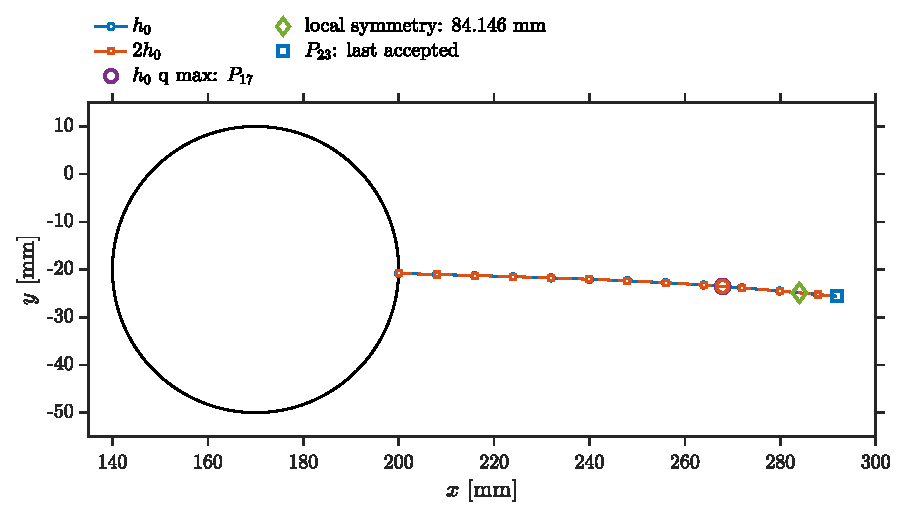
\includegraphics[width=\linewidth]{before/figures/tip_resolution_sensitivity/trajectory.pdf}
    \caption{Trajectories with structured-tip spacings $h_0$ and $2h_0$.}
    \label{fig:tipres-trajectory}
  \end{subfigure}

  \par\smallskip

  \begin{subfigure}[t][83mm][t]{0.315\linewidth}
    \centering
    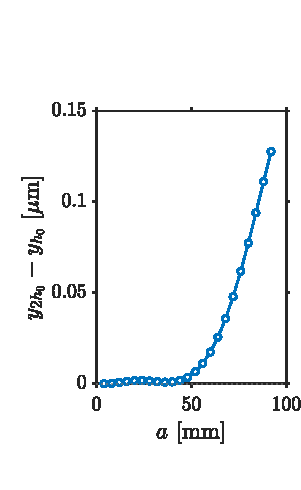
\includegraphics[width=\linewidth]{before/figures/tip_resolution_sensitivity/vertical_deviation.pdf}
    \caption{Accumulated vertical tip-coordinate difference,
    $y_{2h_0}-y_{h_0}$.}
    \label{fig:tipres-dy}
  \end{subfigure}
  \hfill
  \begin{subfigure}[t][83mm][t]{0.315\linewidth}
    \centering
    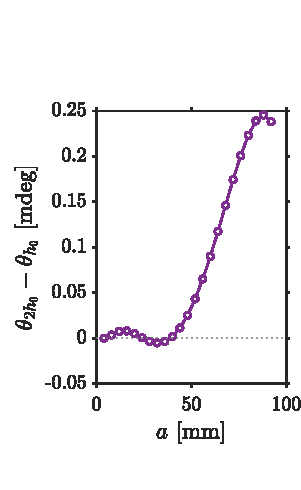
\includegraphics[width=\linewidth]{before/figures/tip_resolution_sensitivity/direction_deviation.pdf}
    \caption{Difference in the absolute crack direction in the frozen initiation frame,
    $\theta_{2h_0}-\theta_{h_0}$.}
    \label{fig:tipres-dtheta}
  \end{subfigure}
  \hfill
  \begin{subfigure}[t][83mm][t]{0.315\linewidth}
    \centering
    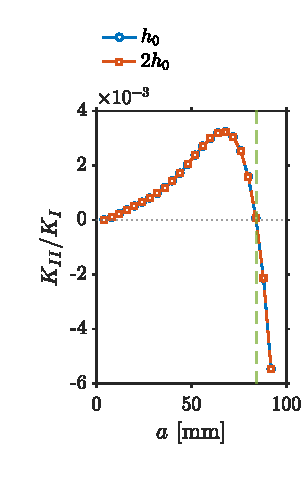
\includegraphics[width=\linewidth]{before/figures/tip_resolution_sensitivity/mode_mixity.pdf}
    \caption{Mode-mixity ratio $K_{\mathrm{II}}/K_{\mathrm{I}}$ along the two independently
    propagated trajectories.}
    \label{fig:tipres-q}
  \end{subfigure}

  \end{minipage}
  \caption{Effect of structured-tip resolution on the propagated
  trajectory. The $h_0$ and $2h_0$ paths share the interaction-domain
  radii and prescribed exterior sizing. The diamond indicates the
  interpolated mode-mixity zero of the reference path.}
  \label{fig:tip-resolution-sensitivity}
\end{figure}
\clearpage
\begin{figure}[tbp]
  \centering
  \begin{minipage}{0.8\textwidth}
  \centering

  \begin{subfigure}[t][86mm][t]{0.94\linewidth}
    \centering
    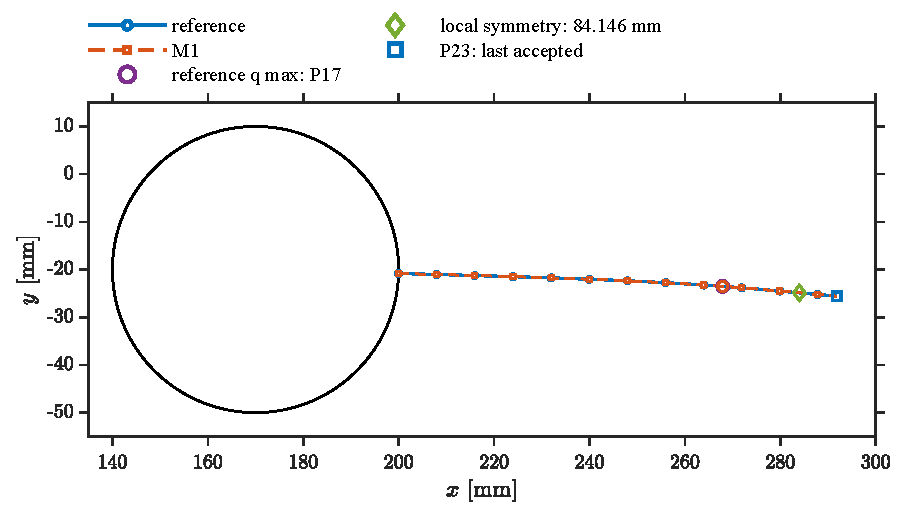
\includegraphics[width=\linewidth]{before/figures/m1_mesh_sensitivity/trajectory.pdf}
    \caption{Crack trajectories with the reference and M1 exterior meshes.}
    \label{fig:m1mesh-trajectory}
  \end{subfigure}

  \par\smallskip

  \begin{subfigure}[t][83mm][t]{0.315\linewidth}
    \centering
    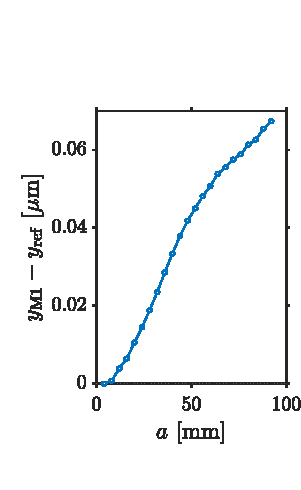
\includegraphics[width=\linewidth]{before/figures/m1_mesh_sensitivity/vertical_deviation.pdf}
    \caption{Accumulated vertical tip-coordinate difference,
    $y_{\mathrm{M1}}-y_{\mathrm{ref}}$.}
    \label{fig:m1mesh-dy}
  \end{subfigure}
  \hfill
  \begin{subfigure}[t][83mm][t]{0.315\linewidth}
    \centering
    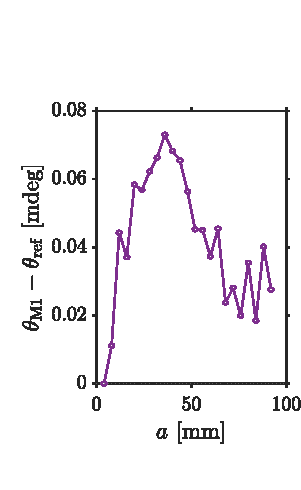
\includegraphics[width=\linewidth]{before/figures/m1_mesh_sensitivity/direction_deviation.pdf}
    \caption{Difference in the absolute crack direction in the frozen initiation frame,
    $\theta_{\mathrm{M1}}-\theta_{\mathrm{ref}}$.}
    \label{fig:m1mesh-dtheta}
  \end{subfigure}
  \hfill
  \begin{subfigure}[t][83mm][t]{0.315\linewidth}
    \centering
    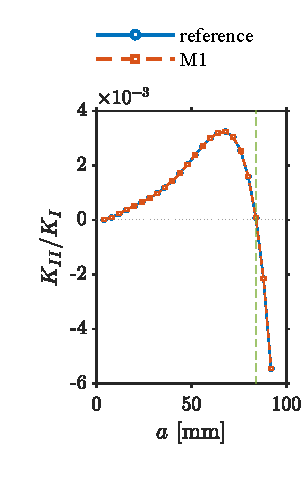
\includegraphics[width=\linewidth]{before/figures/m1_mesh_sensitivity/mode_mixity.pdf}
    \caption{Mode-mixity ratio $K_{\mathrm{II}}/K_{\mathrm{I}}$ along the two independently
    propagated trajectories.}
    \label{fig:m1mesh-q}
  \end{subfigure}

  \end{minipage}
  \caption{Effect of exterior-mesh coarsening on the crack path.
  The reference and M1 trajectories are propagated separately with
  identical near-tip discretizations and interaction-domain radii.
  The diamond marks the interpolated mode-mixity zero of the
  reference path.}
  \label{fig:m1-mesh-sensitivity}
\end{figure}
\clearpage
\begin{figure}[tbp]
  \centering
  \begin{minipage}{0.8\textwidth}
  \centering

  \begin{subfigure}[t]{0.94\linewidth}
    \centering
    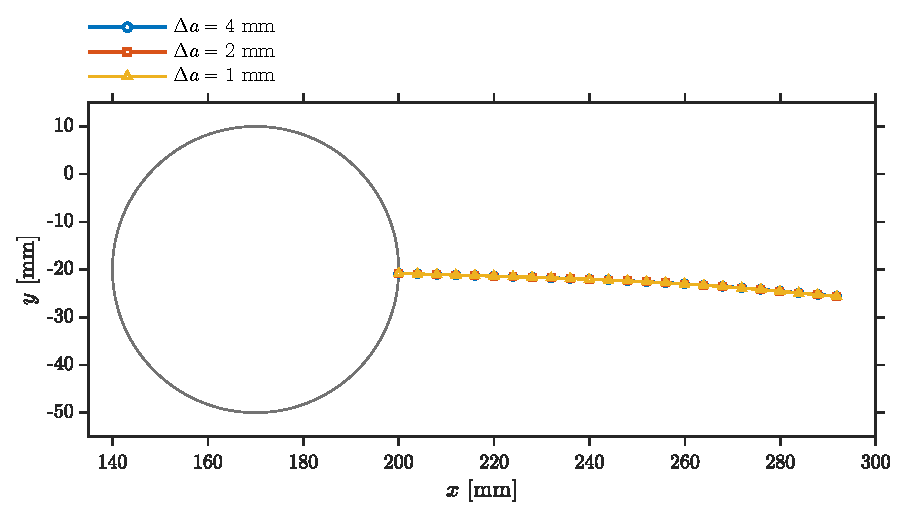
\includegraphics[width=\linewidth]{before/figures/increment_sensitivity/trajectory.pdf}
    \caption{Independently propagated crack trajectories for
    $\Delta a=4$, 2, and 1 mm, all continued to 92 mm.}
    \label{fig:inc-trajectory}
  \end{subfigure}
  \par\smallskip
  \begin{subfigure}[t]{0.315\linewidth}
    \centering
    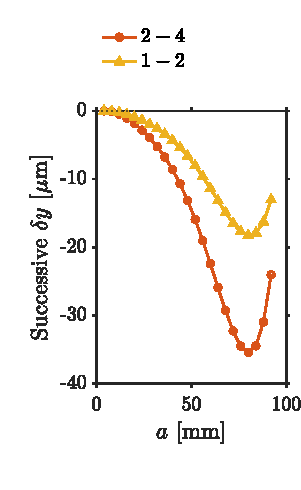
\includegraphics[width=\linewidth]{before/figures/increment_sensitivity/vertical_deviation.pdf}
    \caption{Successive vertical-coordinate differences,
    $y_{2\,\mathrm{mm}}-y_{4\,\mathrm{mm}}$ and
    $y_{1\,\mathrm{mm}}-y_{2\,\mathrm{mm}}$, evaluated at exact
    common crack lengths.}
    \label{fig:inc-dy}
  \end{subfigure}
  \hfill
  \begin{subfigure}[t]{0.315\linewidth}
    \centering
    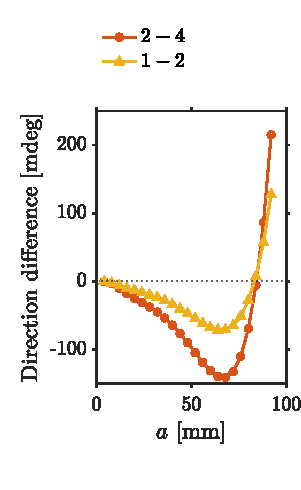
\includegraphics[width=\linewidth]{before/figures/increment_sensitivity/direction_deviation.pdf}
    \caption{Successive differences in absolute crack direction in the
    frozen initiation frame.}
    \label{fig:inc-dtheta}
  \end{subfigure}
  \hfill
  \begin{subfigure}[t]{0.315\linewidth}
    \centering
    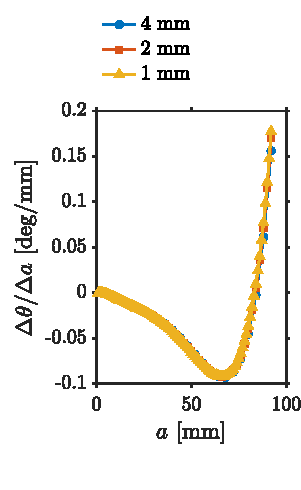
\includegraphics[width=\linewidth]{before/figures/increment_sensitivity/turn_density.pdf}
    \caption{Turning density $\Delta\theta/\Delta a$ along the three
    independently propagated trajectories.}
    \label{fig:inc-turn-density}
  \end{subfigure}

  \end{minipage}
  \par\medskip
  \caption{Coupled crack-increment and discretization refinement.
  The $4$-, $2$-, and $1$-mm paths share dimensionless mesh and
  interaction-domain scales. Panels (b,c) compare paths at common
  crack lengths; panel (d) shows turning density on each path's
  native grid.}
  \label{fig:increment-sensitivity}
\end{figure}\end{document}
